\section{Environmental Impact}

\subsection{Waste prevention and minimisation}

Nitroma is conscious of the adverse effects that our activities may have on the environment. The company strives to set an industry standard for being environmentally sustainable in the chemical manufacture field. The prevention and minimisation of waste are key to achieving this goal. 

\subsubsection{Choice of reducing agent}
The selection of compounds utilised in the various plant reactions allowed waste prevention. For the hydrogenation to 4-aminobenzaldehyde and 4-aminobenzoic acid, a choice was made between two reducing agents, formic acid and ammonium formate. Whist ammonium formate is more favourable in terms of reaction time (the low residence time offering a faster pathway), the use of this reducing agent will produce ammonia as a side product. Acting as a  source of nitration pollution, gaseous ammonia emissions have harmful affects on biodiversity; forming acid deposits in soil, inflicting toxic damage on plants, and negatively altering aquatic ecosystems through a significant nutrient shift \cite{european_environment_agency_ammonia_2019}. Based on this, formic acid was chosen as the reducing agent over ammonium formate, eliminating the unnecessary formation of ammonia. 

\subsubsection{Sulphuric acid and nitrogen oxides}
The nitration reaction process presented an opportunity for waste prevention and minimisation. Traditionally, nitration reactions employ a mixture of nitric acid and sulphuric acid. However, the disposal of 'spent' sulphuric acid has been found to be both costly and environmentally unfriendly. The replacement of sulphuric acid with the zeolite, H-Modernite, provides a more environmentally sustainable nitration pathway. H-Modernite comes with various advantages, including low catalyst loading, its ability to allow short reaction times and its reusable nature. 

%get reference from interim 

Another issue with the use of sulphuric acid in nitration is that it leads to decomposition of nitric acid, forming harmful nitrogen oxides (NOx). Upon the replacement of sulphuric acid with a zeolite catalyst, extensive research was conducted to investigate how NOx may be formed. Our research showed no evidence of NOx emissions from nitration with zeolite catalysts. Nitroma has hypothesised that there is a rapid reaction between the zeolite and the NOx formed from nitric acid decomposition, the resulting product being a nitrating agent which reacts in the nitration itself. Further details on can be found in the synthesis section \ref{sec:synthesis}.2.5. Thus, the use of H-Modernite has allowed prevention of NOx emissions - however if there should be NOx emissions, research suggests this would be less than what would be produced with sulphuric acid. If NOx's are produced, thet will pass through a scrubber before release (see gaseous waste treatment). Thus, through this choice, the minimisation of NOx production via nitration (if not its complete elimination) has been achieved. 

%cross reference to synthesis 

\subsubsection{Recycle and recovery}

Where possible, recycle streams have been integrated into the process, to recover essential reactants. Among the the materials recovered recycle streams are toluene, hydrogen gas, methanol, nitric acid, 2-nitrotoluene and 4-nitrotoluene. Approximately 60\% of nitric acid was recovered, with the remainder undergoing neutralisation (see waste treatment). 


%https://pubs.rsc.org/en/content/articlelanding/1996/cc/cc9960000469/unauth#!divAbstract
%http://www.ajgreenchem.com/article_49085.html


\subsection{Waste Treatment}
\label{sec:waste}

Whilst every effort has been made to prevent and minimise waste, there will inevitably be materials that must be disposed. Nitroma has considered the best techniques available to appropriately treat the various waste streams, ensuring that they comply with the imposed limits. The waste consists of mostly unreacted organic substances, along with spent nitric acid and methanol that was unable to recovered via the recycle. 

\subsubsection{Liquid waste }

Due to the continuous nature of the plant, liquid effluent streams will be continually discharged and so there must be an on-site wastewater treatment plant that is able to manage this demand sufficiently \cite{water_innovations_inc_continuous_2021}.  As seen in table %label the table
the waste streams have high organic content, which is reflected by the high chemical oxygen demand (COD) values of each substance respectively. Each of the waste streams are first collected and stored (table X) showing which streams are stored in the same unit). As W1 contains nitric acid, water will be added to the tank to dilute the stream and ensure that the nitric acid is not concentrated and thus no spontaneous reaction will occur with organic chemicals with the stream. Similarly, W2 contains formic acid and thus will be diluted again to ensure no un


W1 will first undergo neutralisation with lime, reacting the the nitric acid to form calcium nitrate. The outlet from neutralisation will pass through a filter. Here the solid deposits will be retained and sent to landfill, whilst the filtrate will be mixed with W2, before being sent to and stored before being sent to our on-site waste treatment facility. 

%number tables

Various waste treatment methods were investigated, with the performance,  safety of materials involved and economics all taken into account. Options considered included the photo-fenton-oxidation process and wet air oxidation. However these processes were deemed unsuitable due to the flammable nature of some of the components present in the waste streams, including methanol and formic acid. Ultimately, it was decided to use two methods; first adsorption using activated carbon followed by treatment in an anaerobic membrane bioreactor (AnMBR). The adosption process is highly effective in removing organics from the waste streams, reducing the COD by over 90\%. Adsorption is also capable of capturing any inorganics that may be present from the neutralisation process. It has been found that rather than using commercial carbon adsorbents, the use of activated carbon produced by animal horn is a favourable alternative offering a high performance treatment (reducing the COD by 95.67\%) at a lower cost \cite{aluyor_cod_2008}. Following adsorption, the organic waste stream will be sent into the AnMBR for further treatment. AnMBRs offer a low energy input treatment method for waste treatment \cite{maaz_anaerobic_2019}, allowing over 97\% COD removal whilst transforming the organic matter into biogas \cite{ariunbaatar_performance_2021}. The biogas consists mainly of methane, produced via action of anaerobic microorganisms accustomed to a  . Approximately 70\% of organics are converted into methane \cite{ariunbaatar_performance_2021}, whilst the rest is broken down into \ch{CO2}. Configurations of the AnMBR can vary, however it was decided that the membrane module will remain outside the bioreactor itself for better monitoring and maintenance \cite{maaz_anaerobic_2019}. Collaboratively, the use catalytic WAO and AnMBR will be able to reduce the overall COD of the liquid waste effluent below the maximum limit of 250 mg/L. 

% cooling water 

\subsubsection{Gaseous Waste}

In both operation scenarios, there is one stream which contains a gaseous mixture of oxygen and nitrogen. As this stream contains no harmful pollutants, it will be released into the atmosphere. The rest of the gaseous waste streams all contain volatile organic compounds and will thus be disposed of via incineration. The complete combustion of organic compounds is assumed and thus the emission of carbon monoxide and carbon are negligible. To minimise NOx emissions, a low NOx burner will be utilised, favourable due to its NOx removal efficiency (74\%), along with low cost in comparison to other NOx removal methods such as fuel staging and gas recirculation \cite{world_bank_group_pollution_1999}. In addition to this, the flue gas will go through a wet scrubber, with a 99\% efficiency for NOx removal. Through the employment of these methods, the NOx emissions have been limited to 2.78kg/hr during both the BA and BH scenario (below the max 5kg/hr limit) with a total of 18.37t/yr (for 275 days of operation a year). The total \ch{CO2} emissions have been approximated to 1082.50 t/y released, with 174.61kg/hr released during the BH scenario and 91.35kg/hr released during the BA scenario. %need to explain that we operate in two scenarios, BA and BH

To investigate the atmospheric dispersion of \ch{CO2} and \ch{NO2}, the point source Gaussian Plume model was utilised, with the following assumptions made:

\begin{itemize}
\item Constant emission rate of \ch{CO2} and NOx from source
\item Constant wind speed of 3.167m/s (based on the average wind speed in Nanjing, China in the last 13 months)
\item  Effective stack height of 10m 
\end{itemize}

\begin{equation}
C(x,0,0)= \frac{Q}{\pi u_{H} \sigma_{y} \sigma_{z}} \exp\left( \frac{H^2}{2\sigma_{z}^2}\right)
\end{equation}


The \ch{CO2} and \ch{NO2} emissions (in both the BA and the BH scenario), fall below their respective long-term workplace exposure limits (9150mg/m3 and 0.96mg/m3) that are imposed under the COSHH law. The highest concentration of \ch{CO2} occurs during the BH operation, with a peak of 7.94 mg/m3  (under the unstable condition), whilst the highest \ch{NO2} concentration is 0.285mg/m3 under neutral conditions (for both the BA and the BH operation). 

%https://www.hse.gov.uk/pubns/priced/eh40.pdf
\begin{figure*}[t!]
    \centering
    \begin{subfigure}[t]{0.5\textwidth}
        \centering
        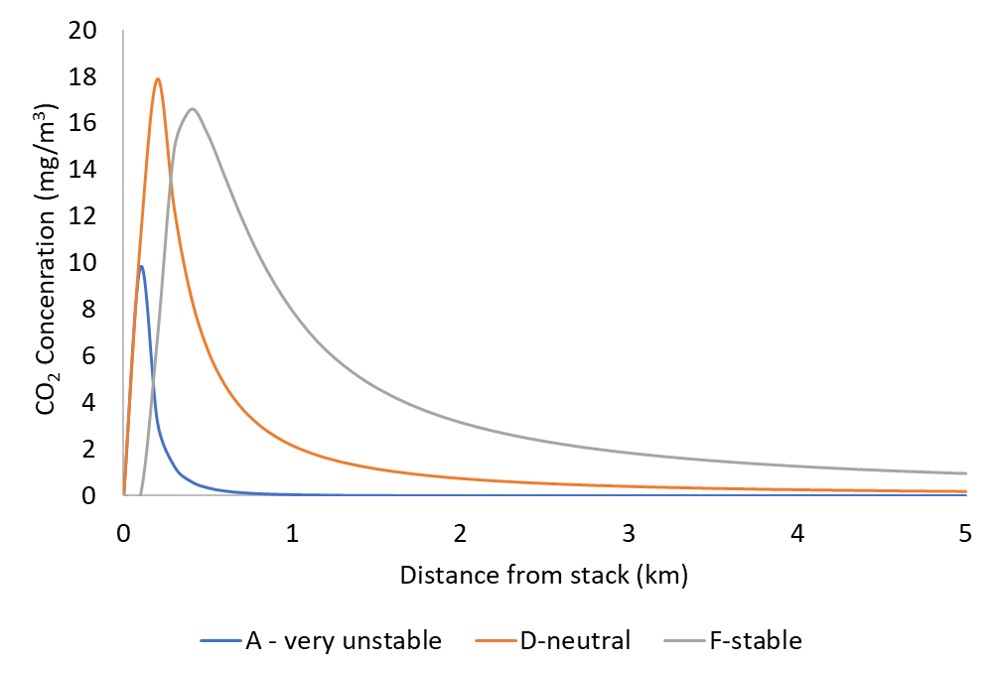
\includegraphics[width=\linewidth]{figures/CO2plume.jpg}
        \caption{$CO_2$ plume model}
    \end{subfigure}%
    ~ 
    \begin{subfigure}[t]{0.5\textwidth}
        \centering
        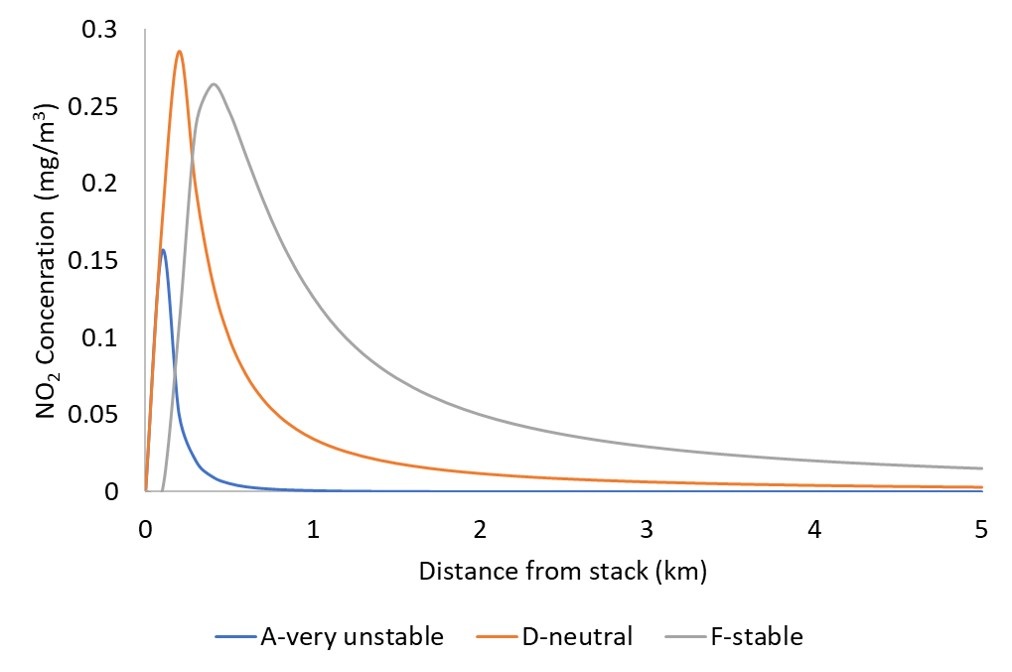
\includegraphics[width=\linewidth]{figures/NO2plume.jpg}
        \caption{$NO_2$ plume model}
    \end{subfigure}
\end{figure*}


\subsection{Greenhouse Gas Emissions}

\begin{wraptable}{r}{0.4\linewidth}
\caption{Greenhouse gas emissions}
\label{tab:GHG}
\begin{tabular}{@{}lllll@{}} \toprule
Emissions (tonnes/year) & \ch{CO2}    & \ch{NO2}  \\ \midrule
Direct                  & 1082.5 & 18.4 \\
Indirect                & 1      &  -     \\
Total                   & 1      &     \\\bottomrule
\end{tabular}
\end{wraptable}

%any recommendations for GHG reduction?

The greenhouse gas emissions from Nitroma's plant are summarised in Table \ref{tab:GHG}. The direct emissions from the incineration of waste streams in the waste treatment area and the indirect emission were from the electricity consumption in the plant for manufacturing the products. 




\subsection{Embodied Energy}

\begin{wraptable}{r}{0.4\linewidth}
\centering
    \caption{Embodied Energy}
    \label{tab:embodied}
\begin{tabular}{@{}lllll@{}}
\toprule
 & Embodied energy (MJ/kg)  \\ \midrule
Raw materials    & 6.643   \\
Transportation     &  0.012  \\
Production                  & 1   \\
Total                  & 1   \\\bottomrule
\end{tabular}
\end{wraptable}

Embodied energy in Nitroma's plant was estimated per kilogram of product manufactured. The energy involved in the extraction of raw material, transportation of the raw material to Nitroma's plant and finally manufacturing the final products are summarised in Table \ref{tab:embodied}. The embodied energy in the raw materials were estimated using heat of reaction and heat of formation for each species. The embodied energy in transportation was determined based on the distance travelled by heavy duty vehicles from the supplier to the plant. Embodied energy in manufacturing the final products in the plant obtained from Business...? 



